\chapter{Atuadores}
Por se tratar de um módulo de fechadura eletrônica, o projeto
apresentará apenas a conexão para que a trava seja colocada.
Dessa forma é possível utilizar qualquer tipo de trava, seja
utilizando solenoides ou eletroímãs \cite{intelbras2019}. Ainda
assim, o circuito de apoio à trava foi feito pelo grupo.

Em geral, há dois tipos de travas, aquelas que estão sempre
fechadas e, ao receber energia elétrica se abrem \cite{madeira2018},
e as que funcionam ao contrário, ficam sempre abertas e se
trancam ao receber a energia \cite{desterro2018}.

Como o circuito auxiliar precisa lidar com os dois casos,
utilizaremos um relé, assim travas que necessitam de energia
para serem fechadas, devem ser ligadas ao terminal normalmente
fechado do relé, e as que se abrem ao receber energia são conectadas
ao terminal normalmente aberto.

Para impedir que o relé queime o controlador são necessários
um resistor e alguns diodos. O resistor diminui a corrente
elétrica que o relé recebe, não permitindo o ATmega  enviar
mais corrente do que ele suporta. Já os diodos impedem que a
corrente induzida pelo relé chegue ao Arduino.

Para finalizar o circuito adicionamos um terminal de três
conectores para a trava. Um dos conectores está ligado no
GND e os outros dois estão ligados um em cada saída do relé,
assim o consumidor pode simplesmente conectar o tipo de trava
que deseja que o módulo acione. O circuito finalizado pode ser
visto na figura ~\ref{fig:esquemaatuador} e o código para seu
funcionamento foi colocado no Apêndice ~\ref{appendix:B}.

\FloatBarrier
\begin{figure}[!htbp]
	\centering
	\caption{Esquema elétrico do teste do atuador}
	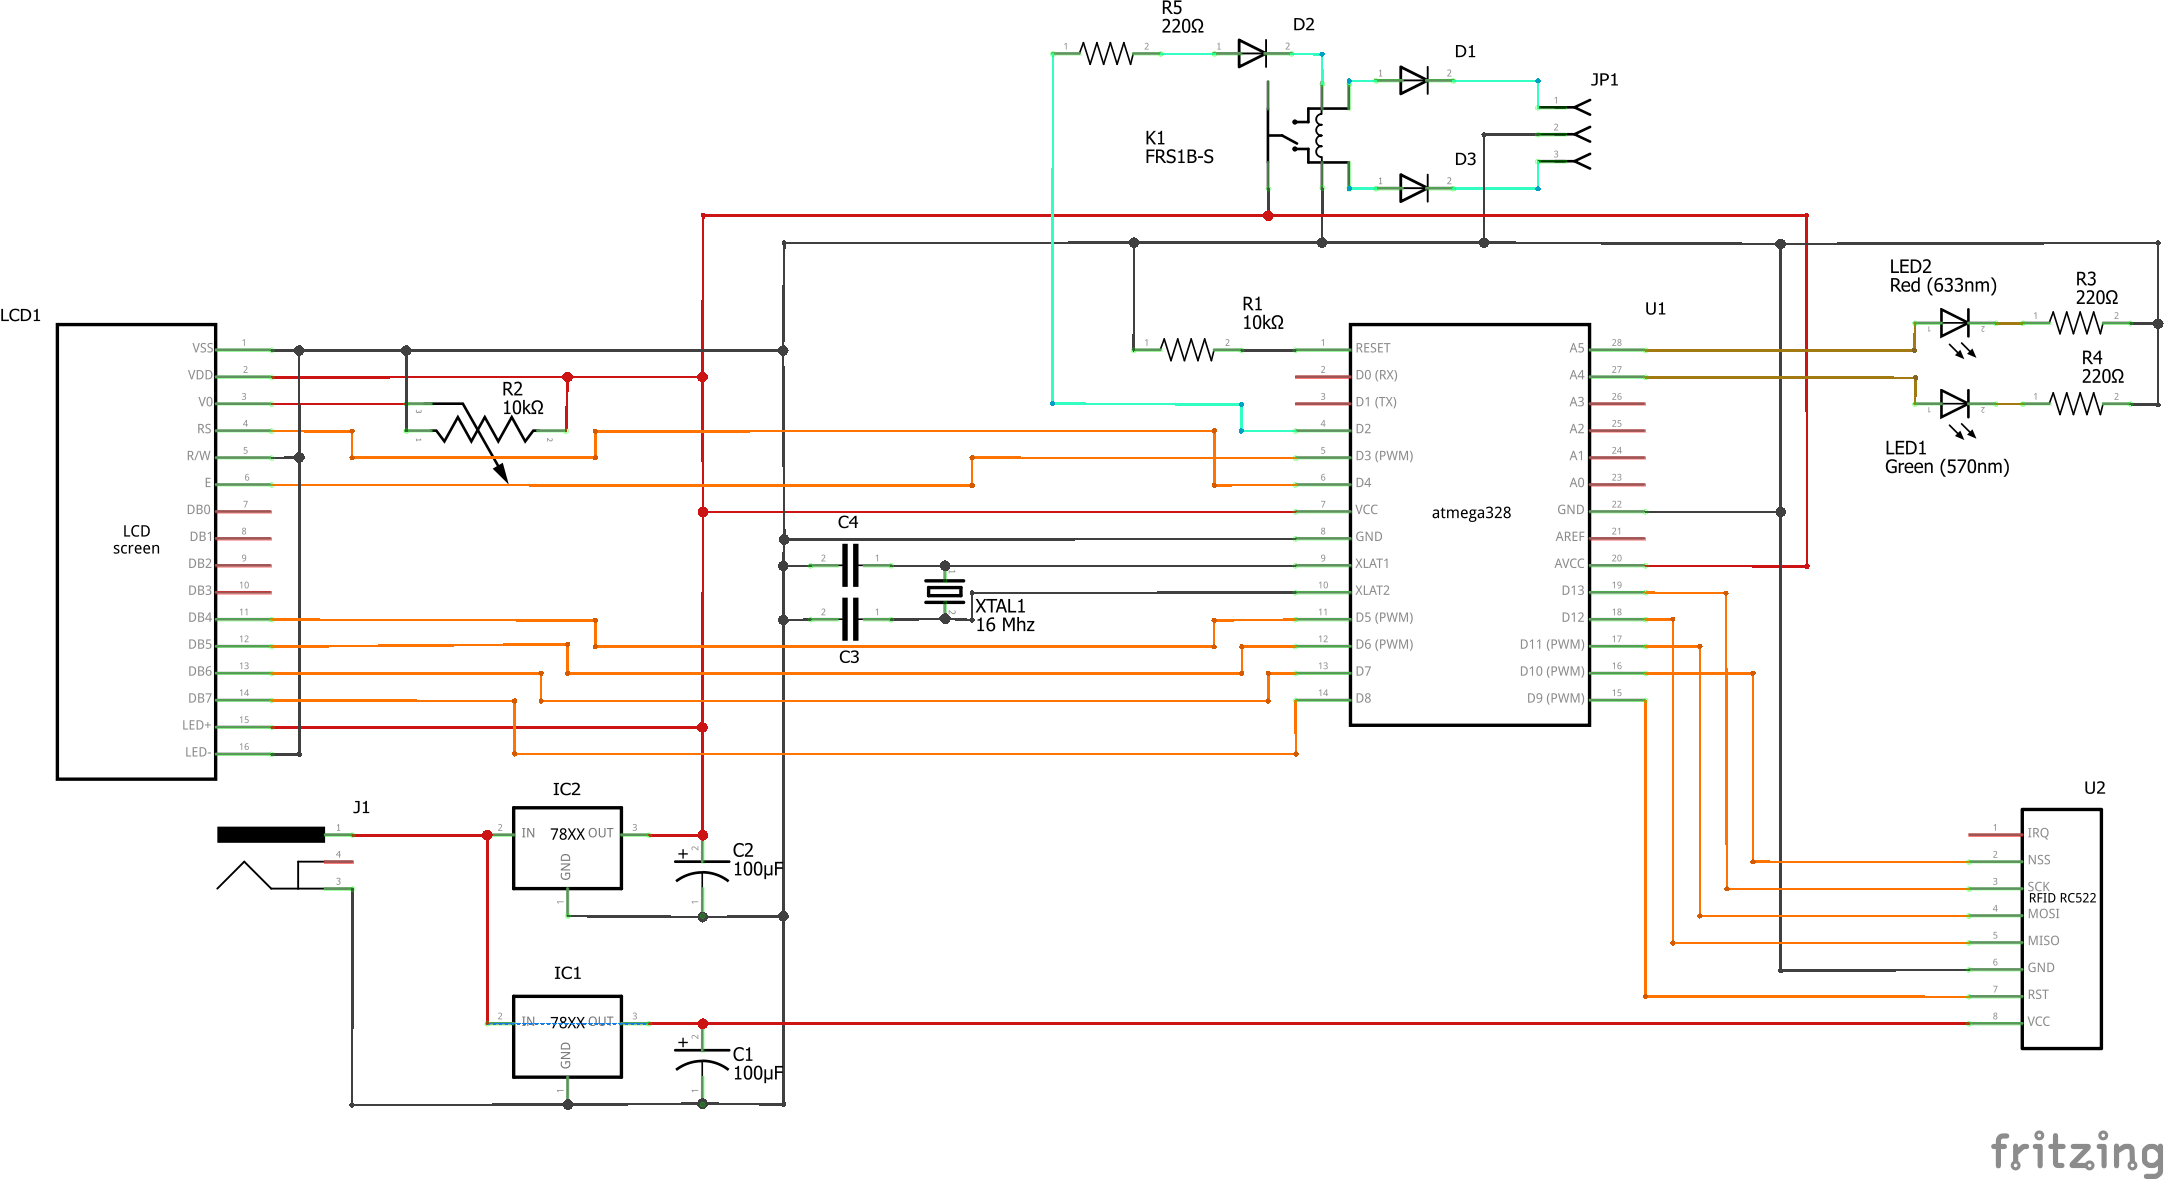
\includegraphics[scale=.6]{imagens/esquemaatuador}
	\\\textbf{Fonte:} Elaborado pelos autores
	\label{fig:esquemaatuador}
\end{figure}
\FloatBarrier